For a fixed scene, let $p$ be the probability of success on one attempt and $G$ the number of independent attempts in a group. A binary group is informative when it contains at least one success and one failure. Its probability is

\begin{equation}
P_{\mathrm{mixed}}=1-(1-p)^G-p^G.
\label{eq:mixed}
\end{equation}

The two subtracted terms are the probabilities that all attempts fail or all attempts succeed. At $p=0.03$ and $G=8$, only 21.6\% of groups contain both outcomes. Dynamic sampling filters uniform groups and collects additional groups within the rollout budget. With dense feedback, the filtering criterion is variation in return; with binary feedback, it is variation in success.

\begin{figure}[!htb]
\centering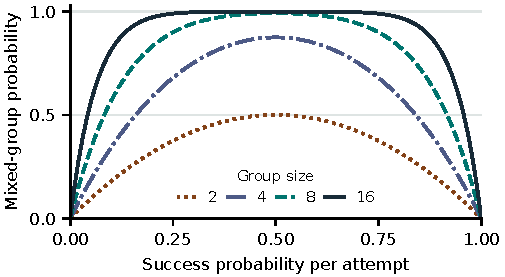
\includegraphics[width=0.95\columnwidth]{figures/mixed_groups.pdf}
\caption{Mixed-outcome probability for group sizes $G=2,4,8,16$. The curves describe independent binary attempts at a fixed scene.}
\label{fig:mixed}
\end{figure}

But the frequency of informative GRPO groups differs from average task success. The expected binary reward is $p$, whereas $P_{\mathrm{mixed}}$ is highest at $p=0.5$ and falls as success approaches one. With binary rewards, group normalization also changes how much each scene contributes to the expected on-policy GRPO update. When scenes share a policy, the resulting objective can favor a small gain in one scene over a larger loss in another~\cite[Sec.~6]{davis2025}.

For example, consider two equally likely scenes and groups of eight attempts. Suppose a policy change raises success in the first scene from 1\% to 2\% and lowers it in the second from 50\% to 48.8\%. The expected fraction of mixed groups rises from 53.47\% to 57.06\%, and the finite-group GRPO objective rises from 0.5381 to 0.5399. Mean task success falls from 25.5\% to 25.4\%.

The numbers illustrate the unfiltered on-policy binary-reward model in~\cite[Sec.~6]{davis2025} in the zero-stabilizer limit.
